%-------------------------------------------------------------------------
% Sample M.Sc. Thesis using the ce class for M.Sc. students computer
% engineering at Delft University of Technology.
% 
% Author: Steven Mulder
% Date:   20/09/2008
%-------------------------------------------------------------------------
%
\documentclass[11pt,twoside,openright,titlepage]{ce}%
%
% define used packages, add your own favorites
%
\usepackage{amsmath,amssymb,amsthm}%
\usepackage{graphicx}%
\usepackage{color}%
\usepackage{listings}%
\usepackage{hyperref}%
%
% set up listings package, for easy code formatting (see example in appendix)
%
\definecolor{darkgreen}{rgb}{0.1333,0.545,0.1333}
\definecolor{darkred}{rgb}{0.698,0,0}
\lstset{basicstyle=\small,%
				tabsize=4,%
				stringstyle=\ttfamily\color{darkred},%
        keywordstyle=\ttfamily\color{blue},%
        identifierstyle=\ttfamily,%
        showstringspaces=false,%
        commentstyle=\ttfamily\color{darkgreen},
        numbers=left,
        stepnumber=5,
        breaklines=true}%
%
% set up hyperref package, for nice clickable references
%
\hypersetup{colorlinks=true,%
            breaklinks=true,%
            linkcolor=black,%
            pdfstartview=FitH,
            pdfpagelayout=TwoColumnRight}%
%
% useful macros
%
\newcommand{\reffig}[1]{Figure~\ref{#1}}%
\newcommand{\reftab}[1]{Table~\ref{#1}}%
\newcommand{\refchap}[1]{Chapter~\ref{#1}}%
\newcommand{\refsec}[1]{Section~\ref{#1}}%
\newcommand{\ie}{i.e.,~}%
\newcommand{\eg}{e.g.,~}%
%
% enter your thesis details
%
\msctitle{My Thesis Title}%
\mscsubtitle{My Subtitle}%
\msckeywords{keywords, msc, thesis, computers, hacking, code}%
\mscauthor{My Name B.Sc.}%
\msccity{My City}%
\msccountry{My Country}%
\mscnumber{00}%
\mscdate{My Graduation Date}%
\major{Computer Engineering}%
\mscinstitute{Delft University of Technology}%
\mscfaculty{Electrical Engineering, Mathematics and Computer Science}%
\mscdepartment{Microelectronics \& Computer Engineering}%
\mscgroup{Circuits and Systems}%
\chairperson{prof.dr.ir. Th.E. Chairperson}%
\advisorone{prof.dr.ir. M.Y. Advisor}%
%\advisortwo{ir. S.E.C. Advisor}%
\memberone{dr. F.R.S.T. Committee-Member}%
\membertwo{dr.ir. S.N.D. Member}%
%\memberthree{ir. Th.R.D. Member}%
%\memberfour{dr. F.Th. Member}%
%
% type your abstract here to have it appear on the cover page and in the Abstract chapter
%
\def\ABSTRACT{%
This is a sample thesis to demonstrate the \texttt{ce} thesis template. The rest of this abstract is filled with random gibberish.

Lorem ipsum dolor sit amet, consectetuer adipiscing elit. Donec varius diam eget ipsum. In rhoncus hendrerit ligula. Fusce dolor. Cras ut velit ut enim fermentum ullamcorper. In tempor justo ut augue. Nullam lacus pede, iaculis eget, facilisis consequat, bibendum sit amet, risus. Sed arcu dui, mattis id, convallis eu, venenatis et, eros. Etiam quis dui id quam aliquam consectetuer. Maecenas metus. Aenean auctor, augue non rutrum commodo, metus dolor mollis diam, vel pellentesque ante augue nec dui. Nullam tellus. Vestibulum vel augue eget turpis euismod tincidunt. Proin nibh lacus, pulvinar non, accumsan in, consectetuer sit amet, lectus. Pellentesque a ligula ac nibh condimentum imperdiet.

Aliquam sodales tortor eget dolor. Donec at nunc. Vestibulum pharetra. Sed posuere. Sed pretium eros vitae quam. Proin accumsan, eros ullamcorper cursus feugiat, orci justo dignissim neque, vehicula pellentesque orci magna a sapien. Etiam magna ligula, volutpat eu, tincidunt eu, ultricies sit amet, pede. Donec metus justo, tristique eget, condimentum et, sodales et, tortor.
}%
%
% uncomment the next line to build only a part of your thesis:
%\includeonly{ack, intro}
%
%-------------------------------------------------------------------------
% End of the preamble, start of the document
%-------------------------------------------------------------------------
\begin{document}%
%
\frontmatter%
% FRONTMATTER: cover, titlepage, signatures, abstract, acknowledgments
\makecover%
\maketitle%
\makesignature%
% Thesis Abstract ----------------------------------------------
%
\nonumchapter{Abstract}%
%
%
% The abstract you put in the preamble will appear here:
%
\ABSTRACT%
%
\cleardoublepage%
%
\nonumchapter{Acknowledgments}
\vskip 1cm
I would like to thank \FIRSTADVISOR, \SECONDMEMBER, \CHAIRPERSON, and \THIRDMEMBER\ for all their help and support during the project.
A special thanks to \SECONDMEMBER\ for often pushing me in the right direction through our numerous white board sessions.
Secondly, I would also like to especially thank \FIRSTADVISOR for being a major help during, and outside of the project.

In addition to this, I would like to thank Cassandra Gr\"utzner and especially 
Dorottya Hauk for their help proof reading the thesis 
and for many good times during the project.

\vskip 2cm
\noindent \AUTHOR \\
\PLACE \\
\DATE
%
\tableofcontents%
\listoffigures%
\listoftables%
%
\mainmatter%
% MAIN MATTER: put your own chapters here
\chapter{Introduction}

This is the introduction of the demonstration thesis for Computer Engineering students. It is written in \LaTeX\ which makes life easy for us. In the introduction you usually introduce the main problem you solve in the following chapters, and present the outline of the thesis. 

\begin{figure}%
\centering%
\includegraphics{style/cas}%
\caption{The Circuits and Systems Logo}%
\label{sample figure}%
\end{figure}

\section{The Main Problem}

The main problem was coming up with enough text for this demo, so you get a good idea of the possibilities. For instance, you can create chapters with nice elaborate headings. When you want to create some structure in your thesis, you can also divide your chapters into sections and subsections and even subsubsections, which all have progressively less elaborate headings.

\subsection{A Subsection}

This subsections serves no purpose other than showing off its header style. In general it makes little sense to split up a section into a single subsection. 

\subsection{The Other Subsection}

So, not to make a fool of myself, is simply add another subsection. Thankfully this subsection is not very long, we do not want to complicate things too much, do we? I think you get the idea now anyway, you can probably guess what happens when you type create a subsubsection\ldots

\section{Outline}

The outline of this thesis is very simple, since it does not really have a proper subject to cover. Instead, it demonstrates some of the possibilities of the \texttt{ce} class, and of \LaTeX\ in general. 

I just noticed that I have not demonstrated the formatting for paragraphs yet. You create a paragraph by leaving a blank line between sentences. If you do not like the standard way \LaTeX handles new paragraphs (\ie with indentation and no empty space between them), try the following:
\begin{verbatim}
\setlength{\parindent}{0pt}
\setlength{\parskip}{1ex plus 0.5ex minus 0.2ex}
\end{verbatim}
This removes the indentation and add a little space between them. Be careful: this also affects the formatting of the Table of Contents!
%
\chapter{First Real Chapter} \label{sample chapter}

I am sorry, this is only a sample chapter so it really has no point except to show you what a chapter looks like in this document style. You should not bother to read all of this, there is no useful information to be found here. Or is there? Have you noticed that \LaTeX\ automatically fixed references for you? The hyperref package, which is activated by default in this thesis class, even creates fancy clickable references, like this one: \reffig{sample figure}.

If you run into any problems with \LaTeX, you might want to take a look at \textit{The Not So Short Introduction to \LaTeX2e}, by Tobias Oetiker. You can find it at the following location: \url{http://tobi.oetiker.ch/lshort/lshort.pdf}.

\section{Advantages}

A strong point is the beautiful way \LaTeX\ typesets math equations. Take a look at the identity, made famous by Euler himself:
\begin{equation}
e^{j\pi} + 1 = 0.
\end{equation}
This is a beautiful equation on its own, but my point is that \LaTeX\ really enables you to easily create equations that look nice and readable.

\section{Disadvantages}

Getting started with \LaTeX\ can be difficult and confusing. Especially the way you add illustrations to your document is awkward. This thesis uses vector-based EPS illustrations, which always look crisp when printed.

However, sometimes you also need to use bitmap pictures like JPG or PNG. Unfortunately you can not use both vector graphics and bitmap graphics in the same document. You actually need a different compiler to process \LaTeX\ with, like pdf\LaTeX. You might want to try and convert you JPGs to EPS using \texttt{xv}, \texttt{convert} or \texttt{jpeg2eps}. The photograph in \reffig{FIG RTG} was converted using \texttt{jpeg2eps}.

Getting started with \LaTeX\ can be difficult and confusing. Especially the way you add illustrations to your document is awkward. This thesis uses vector-based EPS illustrations, which always look crisp when printed.

Getting started with \LaTeX\ can be difficult and confusing. Especially the way you add illustrations to your document is awkward. This thesis uses vector-based EPS illustrations, which always look crisp when printed.

Getting started with \LaTeX\ can be difficult and confusing. Especially the way you add illustrations to your document is awkward. This thesis uses vector-based EPS illustrations, which always look crisp when printed.

\begin{figure}%
\centering%
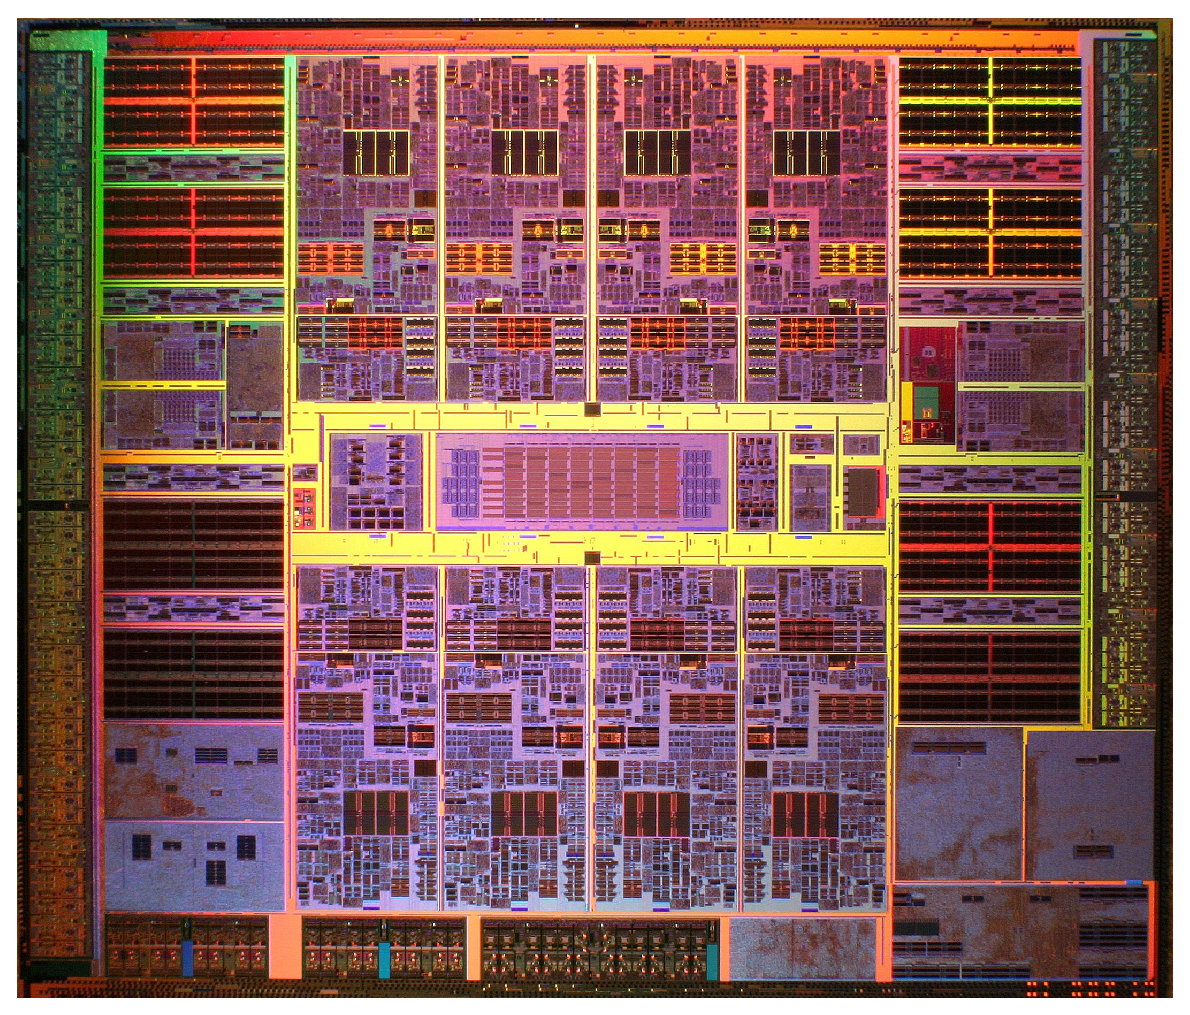
\includegraphics[width=.7\textwidth]{demopic}%
\caption{UltraSparc T2 microprocessor}%
\label{FIG RTG}%
\end{figure} %
%
\appendix%
% APPENDIX: everything that does not belong in the main matter
%-------------------------------------------------------------------------
% Sample use of the listings package. Adapted from the DCSC demo thesis
% 
% Author: Steven Mulder
% Date:   20/09/2008
%-------------------------------------------------------------------------
%
\chapter{Code Examples}

\section{An Appendix Section}

This appendix demonstrates the use of the listings package for displaying programming code in \LaTeX.

\subsection{Some C++ Code}

\lstset{language=C++}
\lstinputlisting{test.c}

\subsection{A MATLAB Listing}

\lstset{language=Matlab}
\lstinputlisting{test.m}%
%
\end{document}
